\chapter{Acceptance Test}
This chapter deals with the needed tests that the system must overcome in order to fulfill the requirements as well as an analysis of the other capabilities, described in \chapref{chap:specifications}.

\section{Requirements Test}

- \textbf{The Cubli should be able to balance starting from an unstable equilibrium position and a null velocity.}

To test this requirement the Cubli is placed at equilibrium and the controller is then started. The test is done twice, with the measurements of the potentiometer and the IMU, to ensure that the controller works in both cases.

\begin{minipage}{\linewidth}
	\begin{minipage}{0.45\linewidth}
		\begin{figure}[H]
			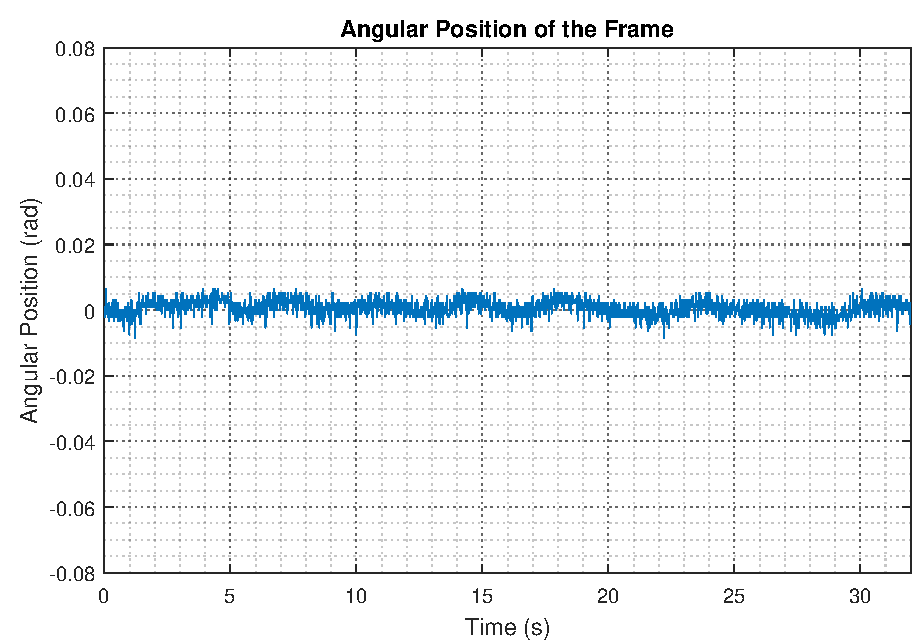
\includegraphics[scale=.45]{figures/testReq1}
			\centering
			\captionsetup{justification=centering}
			\captionof{figure}{Angular position of the frame, measured with the potentiometer, when starting from equilibrium position}
			\label{testReq1}
		\end{figure}
	\end{minipage}
	\hspace{0.03\linewidth}
	\begin{minipage}{0.45\linewidth}
		\begin{figure}[H]\vspace{0mm}
			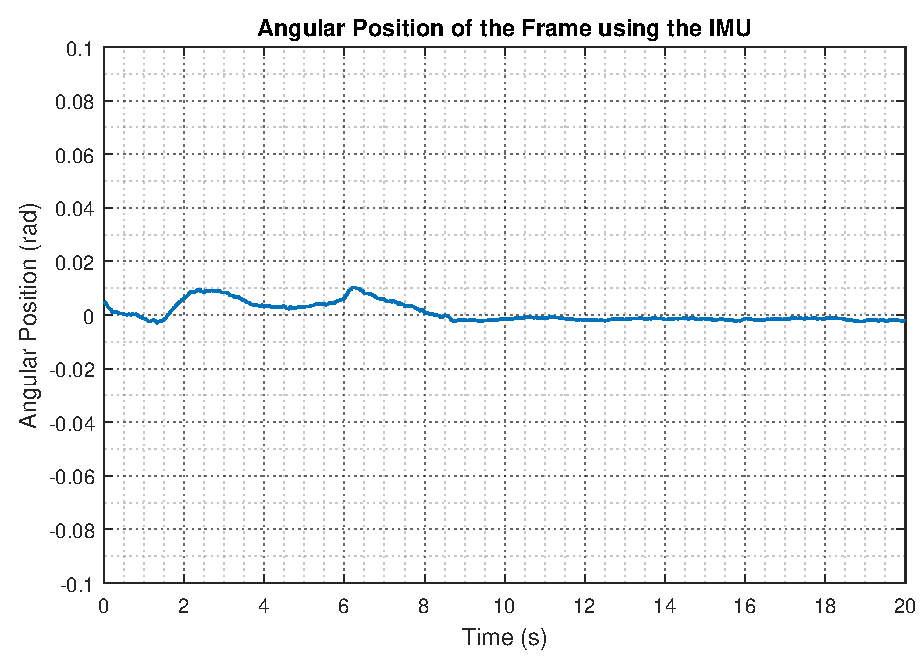
\includegraphics[scale=.45]{figures/testReq1_IMU}
			\centering
			\captionsetup{justification=centering}
			\captionof{figure}{Angular position of the frame starting from equilibrium position, calculated with the complementary filter}
			\label{testReq1_IMU}
		\end{figure}
	\end{minipage}
\end{minipage}
%

The results show that the requirement is fulfilled in both cases since the system is maintained around the equilibrium position.

- \textbf{The prototype should be able to balance around \si{0\ \rad}, even though the angle of inclination of the baseplate is changed within a reasonable range, using internally mounted sensors.}

To check this requirement a similar test, like the previous one, is done, but is this case the angle of the baseplate is changed to check that the measurements of the IMU are still capable of balance the Cubli. Since the potentiometer is attached to the baseplate its measurements are done in relation to the baseplate's position and can be used to show that baseplate and frame are at different angles.

\begin{figure}[H]
	\centering
	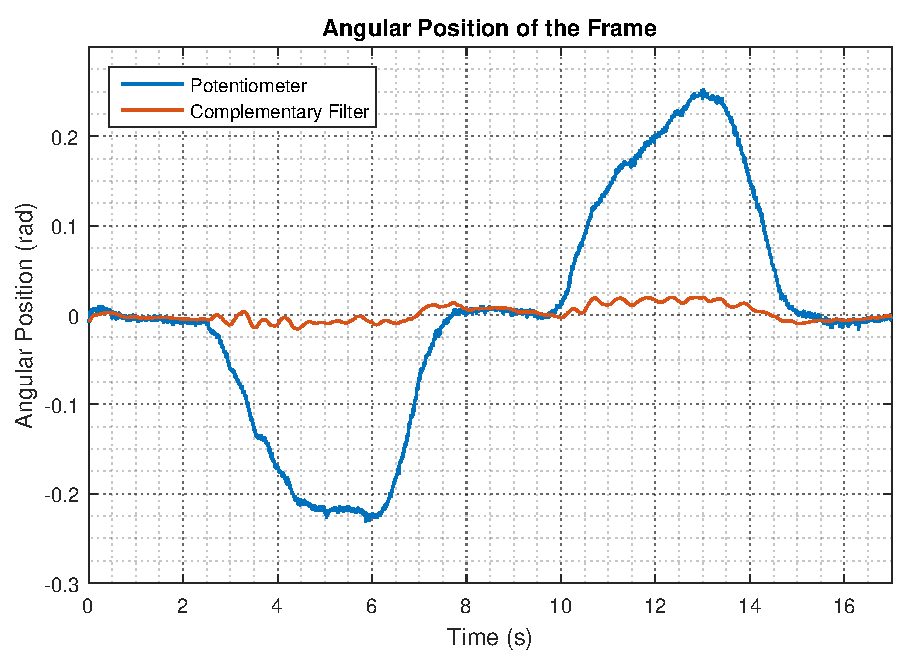
\includegraphics[scale=0.62]{figures/testReq2}
	\caption{Angular position of the frame. The red curve is the result of the complementary filters angle calculation, which does not depend on the angle of the baseplate. The blue curve shows the measurements of the potentiometer, which are in relation to the baseplate.}
	\label{testReq2}
\end{figure}\vspace{-5mm}
%
The output of this experiment shows that the calculation of the position using the IMU makes the system able to keep in equilibrium position when the angle of the Baseplate is changed. This can be seen on the graph in \figref{testReq2}. Here the angle calculated by the complementary filter shows the frame keeping its upright position, while the potentiometer angle changes as the baseplate is lifted up and down. 

\section{Capabilities Analysis}
- \textbf{Maximum recovery angle}

To obtain the maximum recovery angle, the Cubli is place in equilibrium at the start. Once the controller has balance it, its position is changed with little disturbances. The result can be seen in \figref{testRecovery}.

\begin{figure}[H]
	\centering
	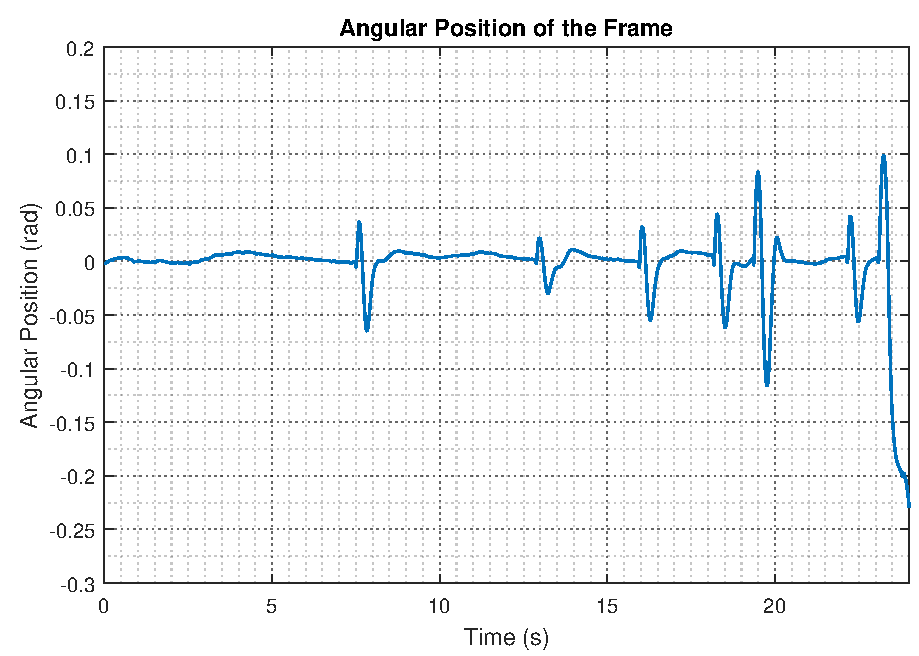
\includegraphics[scale=0.62]{figures/testRecovery}
	\caption{Angular position of the frame while disturbances are applied to the frame. The intention is to find the maximum recovery angle of the controller. The controller is not able to recover from a disturbance that pushes the frame over \SI{0,08}{rad} from resting position, because of overshoot from trying to recover from the disturbance.}
	\label{testRecovery}
\end{figure}\vspace{-5mm}
%
As it can be observed, the controller is able to return to equilibrium position but it creates a remarkable overshoot in the other direction. This behavior limits the recovery angle since the overshoot may drive the Cubli to an angle beyond its handling limit even though the initial disturbance is within it.\\
It can be seen that the controller is capable of recovering from \si{0,08\ rad} but it fails when the angle is \si{0,1\ rad}. Then, it can be concluded that the maximum recovery angle for the system with the designed controller is \si{0,08\ rad}.

- \textbf{Maximum catching angle with no initial velocity of the wheel}

There exists a limitation in this capability which is given by the maximum current that the motor can provide. As can be seen in \figref{limitationTorque}, if the initial angle is different from 0 rad both the mass of the frame and the mass of the wheel exert an initial torque to the system. This must be overcame by the motor to avoid the Cubli to fall.

\begin{figure}[H] 
	\centering
	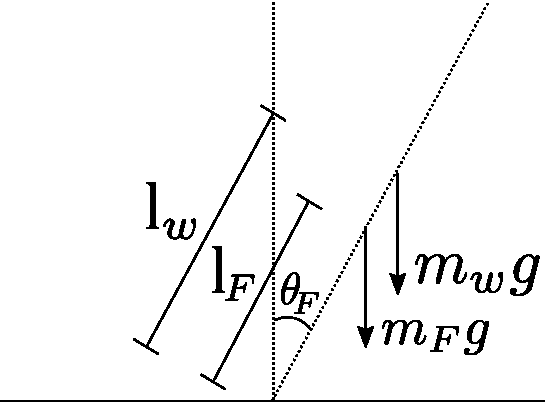
\includegraphics[scale=0.65]{figures/limitationTorque}
	\caption{Forces acting on the system that create an initial torque when the frame starts from a position different from 0 rad}
	\label{limitationTorque}
\end{figure}

The minimum torque (T) that the motor must apply is give by \eqref{minTorque}.
%
\begin{flalign}
	\eq{T} { (m_F \cdot l_F + m_w \cdot l_w) \cdot g \cdot sin(\theta_F)} \unit{N\cdot m}
	\label{minTorque}
\end{flalign}

Since the torque is restricted by the characteristics of the motor and the control board, the maximum initial angle is derived in \eqref{maxAngle}.
%
\begin{flalign}
	\eq{\theta_F} { asin\left(\frac{T}{(m_F \cdot l_F + m_w \cdot l_w) \cdot g}\right)} \unit{rad}
	\label{maxAngle}
\end{flalign}
%
Substituting the values of the maximum torque (see section \secref{sec:Motor}) and the parameters of the Cubli (see section \secref{sec:Param}) the maximum possible starting angle is \si{0,2024\ rad} (\si{1,59^\circ}). This also applies for the negative angle since the limitation of torque is the same but with opposite sign. 

Taking this limit into account some starting angles are tested to check if the controller is able to balance the system with these initial conditions. 

As it can be seen in \figref{testCatch_12} and \figref{testCatch_17}, the controller is capable of moving the system to equilibrium position starting from -0,12 and -0,17 rad (also valid for the positive angles). It is also noteworthy that as the starting angles goes away from the equilibrium the controller takes more time and there is more oscillations in the response.

\begin{minipage}{\linewidth}
	\begin{minipage}{0.45\linewidth}
		\begin{figure}[H]
			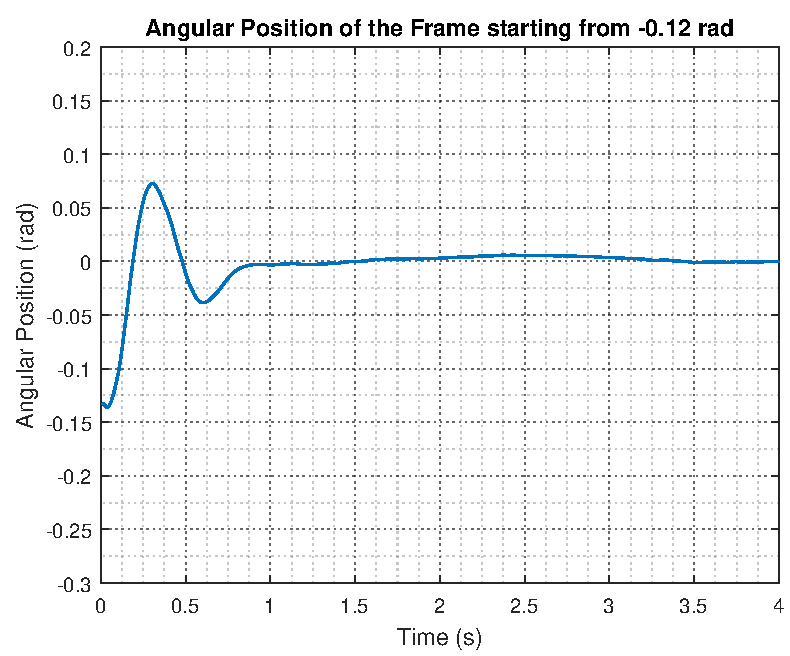
\includegraphics[scale=.55]{figures/testCatch_12}
			\centering
			\captionsetup{justification=centering}
			\captionof{figure}{Angular position of the frame when the system starts from -0,12 rad (\si{-6,87^\circ})}
			\label{testCatch_12}
		\end{figure}
	\end{minipage}
	\hspace{0.03\linewidth}
	\begin{minipage}{0.45\linewidth}
		\begin{figure}[H]\vspace{-3mm}
			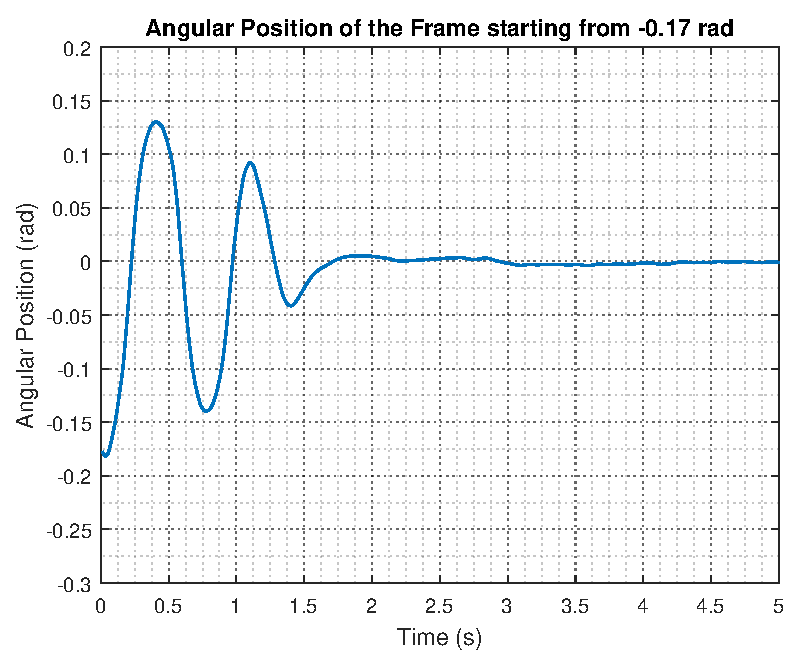
\includegraphics[scale=.55]{figures/testCatch_17}
			\centering
			\captionsetup{justification=centering}
			\captionof{figure}{Angular position of the frame when it starts from -0,17 rad (\si{-9,74^\circ})}
			\label{testCatch_17}
		\end{figure}
	\end{minipage}
\end{minipage}

However, when the starting angle is -0,185 rad (\si{-10,59^\circ}) is no longer possible to balance the system in equilibrium position and the frame falls.

\begin{figure}[H] 
	\centering
	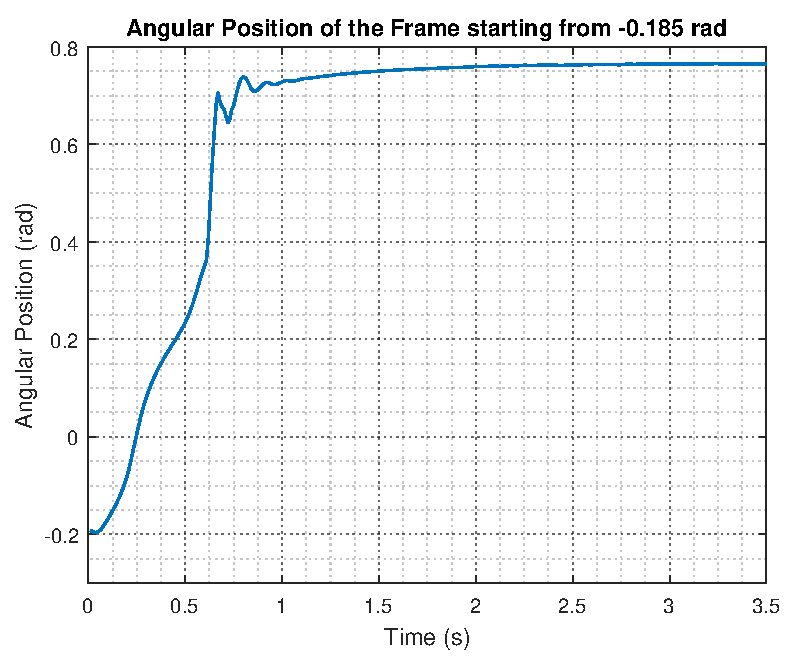
\includegraphics[scale=0.55]{figures/testCatch_185}
	\caption{Angular position of the frame when it starts from -0,185 rad (\si{-10,59^\circ})}
	\label{testCatch_185}
\end{figure}
%
It can be concluded that the maximum range for the starting angle with zero initial conditions goes from -0,17 to 0,17 rad, in which the controller is able to balance the system around equilibrium position.